
%(BEGIN_QUESTION)
% Copyright 2008, Tony R. Kuphaldt, released under the Creative Commons Attribution License (v 1.0)
% This means you may do almost anything with this work of mine, so long as you give me proper credit

In this 480 volt AC induction motor control circuit (sometimes referred to as a ``bucket''), a three-pole relay (typically called a {\it contactor}) is used to switch power on and off to the motor.  The contactor itself is controlled by a smaller switch, which receives 120 volts AC from a step-down transformer to energize the contactor's magnetic coil.  Although this motor control circuit used to work just fine, today the motor refuses to start.

$$\includegraphics[width=15.5cm]{i04449x01.eps}$$

Using your AC voltmeter, you measure 480 volts AC between L1 and L2, 479 volts AC between L2 and L3, and 483 volts AC between L1 and L3.  With the switch in the ``on'' position, you measure 119 volts AC between terminals A1 and A2 on the contactor.  From this information, identify the following:

\vskip 10pt

\begin{itemize}
\item{} \underbar{Two} components or wires in the circuit that you know cannot be failed either open or shorted, besides the 480 volt AC source which is obviously operational.
\vskip 40pt
\item{} \underbar{Two} different component or wire failures in the circuit, either one of which could account for the problem and all measured values, and the types of failures they would be (either open or shorted).
\end{itemize}

\vfil 

\underbar{file i04449}
\eject
%(END_QUESTION)





%(BEGIN_ANSWER)

This is a graded question -- no answers or hints given!

%(END_ANSWER)





%(BEGIN_NOTES)

The fact that we're getting 120 VAC control power all the way to the contactor coil terminals, yet the motor does not start, tells us the problem must lie within the contactor, the three-phase power to the contactor, or within the motor itself.  Since we know we're getting good 480 VAC power between the ``L  terminals, we could be dealing with a fuse failure (but only one where the control power transformer still receives AC power -- thus only the first fuse on L1 could be blown).

\vskip 10pt

\noindent
{\bf Components known to be in good working condition:}

\begin{itemize}
\item{} Both primary windings of the transformer
\item{} Secondary winding of the transformer
\item{} The center (L2) and right (L3) fuses
\item{} All wires from fuses to transformer primary
\item{} Switch
\item{} All wires from contactor to switch to transformer
\end{itemize}

\vskip 10pt

\goodbreak
\noindent
{\bf Components which could possibly be faulted:}

\begin{itemize}
\item{} Contactor coil failed open
\item{} Motor winding(s) failed open
\item{} Wire(s) from fuses to contactor failed open
\item{} Wire(s) from motor to contactor failed open
\item{} L1 fuse blown
\item{} Contactor switch contact(s) failed open
\end{itemize}

%INDEX% Troubleshooting review: electric circuits

%(END_NOTES)


